\documentclass[11pt, oneside]{article}   	% use "amsart" instead of "article" for AMSLaTeX format
\usepackage{geometry}                		% See geometry.pdf to learn the layout options. There are lots.
\geometry{letterpaper}                   		% ... or a4paper or a5paper or ... 
%\geometry{landscape}                		% Activate for for rotated page geometry
%\usepackage[parfill]{parskip}    		% Activate to begin paragraphs with an empty line rather than an indent
\usepackage{graphicx}				% Use pdf, png, jpg, or eps§ with pdflatex; use eps in DVI mode
								% TeX will automatically convert eps --> pdf in pdflatex		
\usepackage{amssymb}
\usepackage{amsmath}
\usepackage{parskip}
\usepackage{color}
\usepackage{hyperref}

\title{Complex sine and cosine}
%\author{The Author}
%\section{}
%\subsection*{}
\date{}							% Activate to display a given date or no date

\graphicspath{{/Users/telliott_admin/Dropbox/Tex/png/}}
% \begin{center} 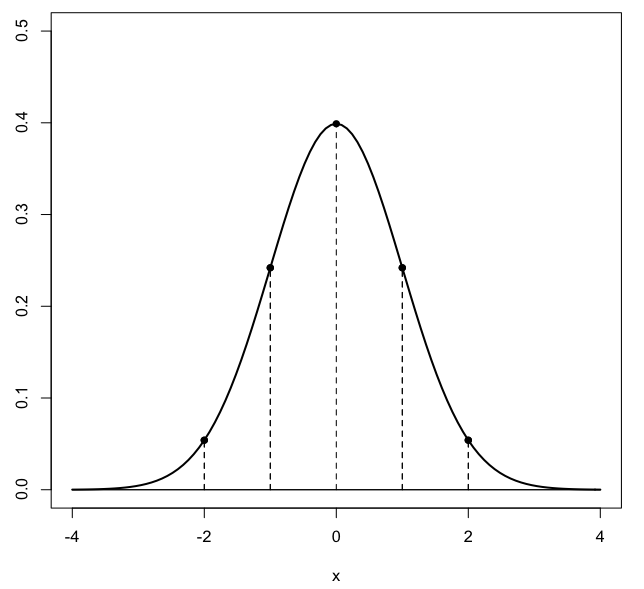
\includegraphics [scale=0.4] {gauss3.png} \end{center}
\begin{document}
\maketitle
\Large

We can define the complex counterparts of the real trigonometric functions by saying that Euler's formula is also good for a complex number $z$ (a math book would define them by their power series).  So
\[ e^{iz} = \cos z + i \sin z \]
and
\[ e^{-iz} = \cos -z + i \sin -z \]
\[ = \cos z - i \sin z \]
This leads to:
\[ \cos z = \frac{1}{2} (e^{iz} + e^{-iz}) \]
and
\[ \sin z = \frac{1}{2i} (e^{iz} - e^{-iz}) \]

A nice property for this definition of cosine is that
\[ \cos z = \frac{1}{2} \ (e^{iz} + e^{-iz}) \]
so
\[ \cos (z + 2\pi) = \frac{1}{2} \ (e^{iz}e^{i2\pi} + e^{-iz}e^{-2\pi}) \]
but
\[ e^{i 2 \pi} = \cos 2 \pi + i \sin 2 \pi = 1 = e^{-i 2 \pi} \]
so
\[ \cos (z + 2\pi) = \cos z \]
The \emph{period} of the complex cosine and sine is $2 \pi$.

Take derivatives
\[ \sin z = \frac{1}{2i} \ (e^{iz} - e^{-iz}) \]
\[ \frac{d}{dz} \ \sin z = \frac{1}{2i} i (e^{iz} + e^{-iz}) = \cos z \]
Similarly
\[ \cos z = \frac{1}{2} \ (e^{iz} + e^{-iz} ) \]
\[ \frac{d}{dz} \ \cos z = \frac{i}{2} \ ( e^{iz} - e^{-iz} ) \]
\[ =- \frac{1}{2i} \ ( e^{iz} - e^{-iz} ) = -\sin z \]

Also
\[ \sin -z = \frac{1}{2i} \ (e^{-iz} - e^{+iz}) = - \sin z \]
\[ \cos -z = \frac{1}{2} \ (e^{-iz} + e^{iz} ) = \cos z \]

\subsection*{hyperbolic connection}
The definitions of the hyperbolic sine and cosine for a real variable are:
\[ \cosh x = \frac{1}{2} (e^x + e^{-x}) \]
\[ \sinh x = \frac{1}{2} (e^x - e^{-x}) \]

Now
\[ \cos z = \frac{e^{iz} + e^{-iz}}{2} \]
if we consider $z = iy$ then
\[ \cos iy = \frac{e^{i^2y} + e^{-i^2y}}{2} \]
\[ = \frac{e^{-y} + e^{y}}{2} \]
But this is just $\cosh y$.  That is:
\[ \cos iy = \cosh y \]
Similarly
\[ 2i \sin iy = e^{i^2y} - e^{-i^2y} \]
\[ = e^{-y} - e^{y} \]
\[ = - (e^y - e^{-y}) \]
\[ = -2 \sinh y \]
Hence 
\[ i \sin i y = -\sinh y \]
\[ \sin i y =  i \sinh y \]

So if we view $z = x + iy$ and use the standard addition formula
\[ \cos z = \cos (x + iy) \]
gives
\[ \cos z = \cos x \cos i y - \sin x \sin i y \]
\[ = \cos x \cosh y - i \sin x \sinh y \]
and what's nice about this is that we have the real and imaginary parts of the complex cosine easily visible.  Similarly
\[ \sin z = \sin(x + iy) \]
\[ = \sin x \cos iy + \cos x \sin iy \]
\[ = \sin x \cosh y + i \cos x \sinh y \]
We could also obtain this result by working through the formulas with the complex exponential.

In fact, that is probably worth doing, since we have not proved yet that the sum of angles formulas are valid for complex numbers.  If we work through starting from Euler it will amount to a proof of that fact.

To prove:
\[ \sin x + iy = \sin x \cos iy + \sin iy \cos x \]
or equivalently
\[ \sin x + iy = \sin x \cosh y + i \sinh y \cos x \]

We had above that:
\[ \sin z = \frac{1}{2i} (e^{iz} - e^{-iz}) \]
and
\[ e^{iz} = e^{i(x + iy)} = e^{ix}e^{-y} \]
\[ e^{-iz} = e^{-i(x+iy)} = e^{-ix} e^y \]

Furthermore
\[ e^{ix} = \cos x + i \sin x \]
\[ e^{-ix} = \cos -x + i \sin -x  = \cos x - i \sin x \]
Putting that all together:
\[ \sin z = \frac{1}{2i} \ [ \ (\cos x + i \sin x)e^{-y} - (\cos x - i \sin x) e^y \ ] \ \]
Group the terms with $\sin x$ together
\[ = \frac{1}{2i} \ [ \ i \sin x (e^{-y} + e^y) + \cos x (e^{-y} - e^y) \ ] \ \]
\[ = \sin x \ \frac{(e^{y} + e^{-y})}{2} -\frac{1}{i} \cos x \frac{(e^{y} - e^{-y})}{i} \]
\[ = \sin x \cosh y + i \cos x \sinh y \]

Cosine is perhaps easier

\[ \cos z = \frac{1}{2} (e^{iz} + e^{-iz}) \]
\[ = \frac{1}{2} \ [ \ (\cos x + i \sin x) e^{-y} + (\cos x - i \sin x) e^y \ ] \]
\[ = \frac{1}{2} \ [ \ (\cos x)(e^y + e^{-y}) + i (\sin x)(e^{y} + e^{-y}) \]
\[ = \cos x \cosh y - \frac{1}{2i} (\sin x)(e^{y} + e^{-y}) \]
now we just massage the second term
\[ = \cos x \cosh y - \frac{1}{i}  \sin x \sinh y \]
\[ = \cos x \cosh y - \frac{1}{i} \sin x (i \sin iy) \]
\[ = \cos x \cosh y - \sin x \sin iy \]

which is what we wanted to prove.

\subsection*{zeroes}

\begin{center} 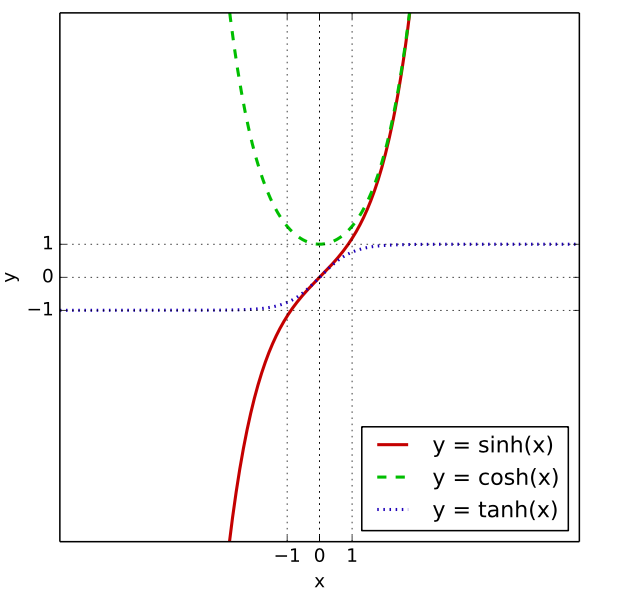
\includegraphics [scale=0.35] {sinhcosh.png} \end{center}
Notice that $\cosh$ is never zero, while only $\sinh 0 = 0$.

So if we look again at 
\[ \sin z = \sin x \cosh y + i \cos x \sinh y \]
and ask, where is this function equal to zero?  

Both parts must vanish.  Since $\cosh$ is never zero, $\sin x$ must be zero.  This happens for $x = 2k \pi$.  

The cosine of this $x$ is equal to $1$, that means $\sinh y$ must be $0$ which only happens for $y = 0$.

So the zeroes of the complex sine function are at $z = 2k \pi + 0i$.

Alternatively, go back to the original definition:
\[ \sin z = \frac{1}{2i} (e^{iz} - e^{-iz}) \]
which vanishes only for 
\[ e^{iz} = e^{-iz} = \frac{1}{e^{iz}} \]
\[ e^{2iz} = \ [ \ e^{iz} \ ]^2 \ = 1 \]
\[ e^{iz} = \pm 1 \]
\[ e^{i(x + iy)} = \pm 1 \]
\[ e^{-y}e^{ix} = \pm 1 \]
\[ e^{-y} (\cos x + i \sin x) = \pm 1 \]
The imaginary part must be zero, so $x = 2k \pi$.  The other part must be equal to $\pm 1$, so $y = 0$ and $\cos 2k \pi = 1$, which works.

For the cosine
\[ \cos z = \frac{1}{2i} (e^{iz} + e^{-iz}) \]
This is equal to zero when
\[ e^{iz} = - e^{-iz} = -\frac{1}{e^{iz}} \]
\[ e^{2iz} = -1 \]
\[ e^{i(x + iy)} = \pm i \]
\[ e^{-y} (\cos x + i \sin x) = \pm i \]
In this case we need $\cos x = 0$ and then $y=0$ and $\sin x = 1$ will work.  $x = (2k + 1)\pi / 2$.

Recall that
\[ \cos z = \cos x \cosh y - i \sin x \sinh y \]
Since $\cosh$ is never zero, $\cos x$ must be zero.  Then either $\sin x = 0$ or $\sinh y = 0$.  Only the latter works for the non-imaginary part, so we have that $y = 0$.

\subsection*{analyticity}
We proved before that the complex exponential is analytic.  There is a theorem that says that if we add two analytic functions together, the result is also analytic.  Hence, the trigonometric functions are analytic.

But, just to check this result, let's write them out in terms of $u$ and $v$ and see whether the partial derivatives follow the CRE conditions:

\[ \sin z = \sin x \cosh y + i \cos x \sinh y \]
Taking the derivatives:
\[ u(x,y) =  \sin x \cosh y \]
\[ u_x = \cos x \cosh y \]
\[ u_y = \sin x \sinh y \]
and
\[ v(x,y) = \cos x \sinh y \]
\[ v_x = - \sin x \sinh y \]
\[ v_y = \cos x \cosh y \]
So we see that
\[ u_x = v_y \]
\[ u_y = -v_x \]

The CRE are satisfied and therefore, the complex sine is analytic.

Similarly we have that 
\[ \cos z = \cos (x + iy) \]
\[ = \cos x \cos iy - \sin x \sin iy \]
\[ = \cos x \cosh y - i \sin x \sinh y \]
So
\[ u(x,y) =  \cos x \cosh y \]
\[ u_x = - \sin x \cosh y \]
\[ u_y = \cos x \sinh y \]
and
\[ v(x,y) = -\sin x \sinh y \]
\[ v_x = -\cos x \sinh y \]
\[ v_y = -\sin x \cosh y \]
So we see that
\[ u_x = v_y \]
\[ u_y = v_x \]
Thus the complex cosine is also analytic.

We can also prove that:

\[ \sin^2 z + \cos^2 z = 1 \]
The easy way is
\[ \cos^2 z + \sin^2 z = \ [ \frac{e^{iz} + e^{-iz}}{2} \ ]^2 +  [ \frac{e^{iz} - e^{-iz}}{2i} \ ]^2 \ ] \]
\[= \frac{e^{2iz} + 2 + e^{-2iz} - e^{2iz} + 2 - e^{-2iz} }{4} \]
\[ = 1 \]

\subsection*{series}
On the other hand, Shankar defines the trig functions and the exponential using series in the same way as the real versions:

\[ \sin z = \sum_0^{\infty} (-1)^n \frac{z^{2n+1}}{(2n +1)!} \]
\[ \cos z = \sum_0^{\infty} (-1)^n \frac{z^{2n}}{(2n)!} \]
\[ \sinh z = \sum_0^{\infty} \frac{z^{2n+1}}{(2n +1)!} \]
\[ \cosh z = \sum_0^{\infty} \frac{z^{2n}}{(2n)!} \]
and showing that they converge for any $z$.

\subsection*{alternate derivation for hyperbolic formula}
\[ \cos z = \frac{1}{2} \ [ \ e^{z} + e^{-z} \ ]  \]
\[ = \frac{1}{2} \ [ \ e^{i(x+iy)} + e^{-i(x + iy)} \ ]  \]
\[ = \frac{1}{2} \ [ \ e^{ix - y} + e^{-ix + y} \ ]  \]
Double the top and the bottom
\[ = \frac{1}{4} \ [ \ e^{ix - y} + e^{-ix + y} + e^{ix - y} + e^{-ix + y}  \ ]  \]
The pattern in the exponents is $+- \ \ -+ \ \ +- \ \ -+$.  

We reach a new pattern by first switching the order to $-+ \ \ +- \ \ -+ \ \ +-$ 
\[ = \frac{1}{4} \ [ \  e^{-ix + y} + e^{ix - y} + e^{-ix + y}  + e^{ix - y} \ ]  \]
then add and subtract terms with $++$ and $--$, like this:
\[ ++ \ -+ \ +- \ -- \ ++ \ -+ \ +- \ -- \]
Written out, we have:
\[ = \frac{1}{4} \ [ \  e^{ix + y} + e^{-ix + y} + e^{ix - y} + e^{-ix - y} - e^{ix + y} + e^{-ix + y}  + e^{ix - y} - e^{-ix - y} \ ]  \]
Group the second set of four terms and put a minus sign out front
\[ = \frac{1}{4} \ [ \  e^{ix + y} + e^{-ix + y} + e^{ix - y} + e^{-ix - y} \ ] - \frac{1}{4} \ [ \ e^{ix + y} - e^{-ix + y}  - e^{ix - y} + e^{-ix - y} \ ]  \]

Now we realize that we can factor the first term as:
\[ = \frac{1}{2}(e^y + e^{-y}) \ \frac{1}{2} (e^{ix} + e^{-ix}) \]
\[ = \cosh y \cos x \]
The second term is:
\[ = - \frac{1}{2}(e^y - e^{-y}) \ \frac{1}{2} (e^{ix} - e^{-ix}) \]
\[ = -i \frac{1}{2}(e^y - e^{-y}) \ \frac{1}{2i} (e^{ix} - e^{-ix}) \]
\[ = -i \sinh y \sin x \]

Putting it all together:
\[ \cos z = \cos x \cosh y - i \sin x \sinh y \]
That required a lot of bookkeeping, and now we have to go back and repeat it all for the sine.  So I prefer the derivation that was given previously.

\end{document}  